\chapter{Design of CI PRNG}
\label{Design of CI PRNG}
\minitoc
The designs of our two versions of CI pseudorandom number generators based on discrete chaotic iterations, satisfying Devaney's chaos, are proposed and discussed. Detail operations of this approach are described in this chapter, while their performance and a comparative study will be presented latter.


\section{The generation of pseudorandom sequence}
\label{The generation of pseudorandom sequence}
\subsection{The logistic map}

%Generating a pseudorandom sequence from the orbit of a real chaotic system requires mapping the state of the system to integer domain. Various methods have been proposed for the conversion of a real sequence into an integer sequence, two of them are recalled bellow.

The logistic map, given by:
\begin{center}
$x^{n+1}=\mu ~ x^{n}(1-x^{n})$, with $x^{0}\in(0,1)$, $\mu \in(3.99996,4]$,
\end{center}

\noindent was originally introduced as a demographic model by Pierre Fran\c cois Verhulst in 1838. In 1947, Ulam and Von Neumann ~\cite{ulam1947} studied it as a PRNG. This essentially requires mapping the states of the system $\left(x^n\right)_{n \in \mathds{N}}$ to $\{0,1\}^\mathds{N}$. A simple way for turning $x^n$ to a discrete bit symbol $r$ is by using a threshold function as it is shown in Algorithm~\ref{logisticmap1}.
A second usual way to obtain an integer sequence from a real system is to chop off the leading bits after moving the decimal point of each $x$ to the right, as it is obtained in Algorithm~\ref{logisticmap2}.

\begin{algorithm}
\textbf{Input:} the internal state $x$ (a decimal number)\\
\textbf{Output:} $r$ (a 1-bit word)
\begin{algorithmic}[1]
\STATE$x\leftarrow{4x(1-x)}$
\IF{$x\textless0$}
{
\STATE$r\leftarrow0$;	
}
\ELSE
{
\STATE$r\leftarrow1$;	
}\ENDIF
\STATE return $r$\;
\medskip
\caption{An arbitrary round of logistic map 1}
\label{logisticmap1}
\end{algorithmic}
\end{algorithm}

\begin{algorithm}
\textbf{Input:} the internal state $x$ (a decimal number)\\
\textbf{Output:} $r$ (an integer)
\begin{algorithmic}[1]
\STATE$x\leftarrow{4x(1-x)}$
\STATE$r\leftarrow{\lfloor10000000x\rfloor}$
\STATE return $r$\;
\medskip
\caption{An arbitrary round of logistic map 2}
\label{logisticmap2}
\end{algorithmic}
\end{algorithm}


\subsection{XORshift}
\label{XORshift}

XORshift is a category of very fast PRNGs designed by George Marsaglia~\cite{Marsaglia2003}.
It repeatedly uses the transform of \emph{exclusive or} (XOR) on a number with a bit shifted version of it. The state of a XORshift generator is a vector of bits. At each step, the next state is obtained by applying a given number of XORshift operations to $w$-bit blocks in the current state, where $w = 32$ or $64$. A XORshift operation is defined as follows. Replace the $w$-bit block by a bitwise XOR of the original block, with a shifted copy of itself by $a$ positions either to the right or to the left, where $ 0 < a < w$. This Algorithm~\ref{XORshift} has a period of $2^{32}-1=4.29\times10^9$.


\begin{algorithm}
\textbf{Input:} the internal state $z$ (a 32-bits word)\\
\textbf{Output:} $y$ (a 32-bits word)
\begin{algorithmic}[1]

\STATE$z\leftarrow{z\oplus{(z\ll13)}}$;
\STATE$z\leftarrow{z\oplus{(z\gg17)}}$;
\STATE$z\leftarrow{z\oplus{(z\ll5)}}$;
\STATE$y\leftarrow{z}$;
\STATE return $y$\;
\medskip
\caption{An arbitrary round of XORshift algorithm}
\label{XORshift}
\end{algorithmic}
\end{algorithm}

\subsection{ISAAC}
ISAAC is an array-based PRNG and a stream cipher designed by Robert Jenkins (1996) to be cryptographically secure~\cite{Jenkins1996}. The name is an acronym for Indirection, Shift, Accumulate, Add and Count. The ISAAC algorithm has similarities with RC4. It uses an array of 256 32-bit integers as the internal state, writing the results to another 256-integer array, from which they are read one at a time until empty, at which point they are recomputed. Since it only takes about 19 32-bit operations for each 32-bit output word, it is extremely fast on 32-bit computers.\newline
We give the key-stream procedure of ISAAC in Algorithm~\ref{ISAAC}. The internal state is $x$, the output array is $r$, and the inputs $a$, $b$, and $c$ are those computed in the previous round. % So we need the initial values of a,b, and c. Yes.
The value $f(a,i)$ in Table~\ref{ISAAC} is a 32-bit word, defined for all $a$ and $i\in\{0,\dots,255\}$ as:

\begin{equation}
f(a,i) = \left\{\begin{array}{ll}
a\ll13 & \text{if } i\equiv0~mod~4 , \\
a\gg6 & \text{if } i\equiv1~mod~4 , \\
a\ll2 & \text{if } i\equiv2~mod~4 , \\
a\gg16 & \text{if } i\equiv3~mod~4 . \\
\end{array}
\right.
\end{equation}

\begin{algorithm}
\textbf{Input:} $a$, $b$, $c$, and the internal state $x$\\
\textbf{Output:} an array $r$ of 256 32-bit words
\begin{algorithmic}[1]
\STATE$c\leftarrow{c+1}$;
\STATE$b\leftarrow{b+c}$;
\WHILE{$i=0,\dots,255$}
\STATE$s\leftarrow{x_i}$;
\STATE$a\leftarrow{f(a,i)+x_{(i+128)~mod~256}}$;
\STATE$x_i\leftarrow{a+b+x_{(x\gg2)~mod~256}}$;
\STATE$r_i\leftarrow{s+x_{(x_i\gg10)~mod~256}}$;
\STATE$b\leftarrow{r_i}$;
\ENDWHILE
\STATE return $r$\;
\medskip
\caption{An arbitrary round of ISAAC algorithm}
\label{ISAAC}
\end{algorithmic}
\end{algorithm}

\section{A Theoretical Proof for Devaney's Chaotic Dynamical Systems}
\label{A theoretical proof for Devaney's chaotic dynamical systems}
The outline proofs, of the properties on which our PRNG is based, are given in this section. 

\subsection{A topological approach for chaotic iterations}

Denote by $\delta $ the \emph{discrete boolean metric}, $\delta
(x,y)=0\Leftrightarrow x=y.$ Given a function $f$, define the function $%
F_{f}:$ $\llbracket1;\mathsf{N}\rrbracket\times \mathds{B}^{\mathsf{N}%
}\longrightarrow \mathds{B}^{\mathsf{N}}$ such that $$F_{f}(k,E)=\left(
E_{j}.\delta (k,j)+f(E)_{k}.\overline{\delta (k,j)}\right) _{j\in \llbracket%
1;\mathsf{N}\rrbracket},$$ where + and . are the boolean addition and product operations.

Consider the phase space: $\mathcal{X}=\llbracket1;\mathsf{N}\rrbracket^{%
\mathds{N}}\times \mathds{B}^{\mathsf{N}}$ and the map $$G_{f}\left( S,E\right) =\left( \sigma
(S),F_{f}(i(S),E)\right) ,$$ then the chaotic iterations defined in (\ref{Chaotic iterations}) can be described by the following iterations \cite{guyeux09}
\[
\left\{
\begin{array}{l}
X^{0}\in \mathcal{X} \\
X^{k+1}=G_{f}(X^{k}).%
\end{array}%
\right.
\]

Let us define a new distance between two points $(S,E),(\check{S},\check{E})\in
\mathcal{X}$ by $$d((S,E);(\check{S},\check{E}))=d_{e}(E,\check{E})+d_{s}(S,%
\check{S}),$$ where
\begin{itemize}
\item $\displaystyle{d_{e}(E,\check{E})}=\displaystyle{%
\sum_{k=1}^{\mathsf{N}}\delta (E_{k},\check{E}_{k})} \in \llbracket 0 ; \mathsf{N} \rrbracket$ \\
\item $\displaystyle{%
d_{s}(S,\check{S})}=\displaystyle{\dfrac{9}{\mathsf{N}}\sum_{k=1}^{\infty }%
\dfrac{|S^{k}-\check{S}^{k}|}{10^{k}}} \in [0 ; 1].$
\end{itemize}

\medskip

It is then proven in \cite{guyeux09} by using the sequential continuity that



\begin{proposition}
\label{continuite} $G_f$ is a continuous function on $(\mathcal{X},d)$.
\end{proposition}

\subsection{Regularity}

\label{regularite}

\begin{theorem}
Periodic points of $G_{f}$ are dense in $\mathcal{X}$.
\end{theorem}

\begin{proof}
Let $(S,E)\in \mathcal{X}$, and $\varepsilon >0$. We are looking for a
periodic point $(S^{\prime },E^{\prime })$ satisfying $d((S,E);(S^{\prime
},E^{\prime }))<\varepsilon$.

We choose $E^{\prime }=E$, and we reproduce enough entries from $S$ to $%
S^{\prime }$ so that the distance between $(S^{\prime },E)$ and $(S,E)$ is
strictly less than $\varepsilon $: a number $k=\lfloor log_{10}(\varepsilon
)\rfloor +1$ of terms is sufficient.\newline
After this $k^{th}$ iterations, the new common state is $\mathcal{E}$, and
strategy $S^{\prime }$ is shifted of $k$ positions: $\sigma ^{k}(S^{\prime })$.\newline
Then we have to complete strategy $S^{\prime }$ in order to make $(E^{\prime
},S^{\prime })$ periodic (at least for sufficiently large indices). To do
so, we put an infinite number of 1 to the strategy $S^{\prime }$.

Then, either the first state is conserved after one iteration, so $\mathcal{E%
}$ is unchanged and we obtain a fixed point. Or the first state is not
conserved, then: if the first state is not conserved after a second
iteration, then we will be again in the first case above (due to the fact that a state is a boolean). Otherwise the first state is conserved, and we have
indeed a fixed (periodic) point.

Thus, there exists a periodic point into every neighbourhood of any point, so 
$(\mathcal{X},G_f)$ is regular, for any map $f$.
\end{proof}

\subsection{Transitivity}

\label{transitivite} Contrary to the regularity, the topological
transitivity condition is not automatically satisfied by any function \newline ($
f=Identity$ is not topologically transitive). Let us denote by $\mathcal{T}$
the set of maps $f$ such that $(\mathcal{X},G_{f})$ is topologically
transitive.

\begin{theorem}
$\mathcal{T}$ is a nonempty set.
\end{theorem}

\begin{proof}
We will prove that the vectorial logical negation function $f_{0}$

\begin{equation}
\begin{array}{rccc}
f_{0}: & \mathds{B}^{\mathsf{N}} & \longrightarrow & \mathds{B}^{\mathsf{N}}
\\ 
& (x_{1},\hdots,x_{\mathsf{N}}) & \longmapsto & (\overline{x_{1}},\hdots,%
\overline{x_{\mathsf{N}}}) \\ 
&  &  & 
\end{array}
\label{f0}
\end{equation}%
\noindent is topologically transitive.\newline
Let $\mathcal{B}_A=\mathcal{B}(X_{A},r_{A})$ and $\mathcal{B}_B=\mathcal{B}(X_{B},r_{B})$ be two
open balls of $\mathcal{X}$, where $X_A=(S_A,E_A)$, and $X_B=(S_B,E_B)$. Our goal is to start from a point of $\mathcal{B}_A$ and to arrive, after some iterations of $G_{f_0}$, in $\mathcal{B}_B$.\newline
We have to be close to $X_{A}$, then the starting state $E$ must be $E_{A}$; it
remains to construct the strategy $S$. Let $S^n = S_{A}^n, \forall n \leqslant n_0$, where $n_0$ is chosen in such a way that $(S,E_{A})\in \mathcal{B}_{A}$, and $E'$ be the state of $G_{f_0}^{n_0}(S_{A},E_{A})$.\newline
$E'$ differs from $E_{B}$ by a finite number of cells $c_1,\hdots, c_{n_1}$. Let $S^{n_0+n} = c_n, \forall n \leqslant n_1$. Then the state of $G_{f_0}^{n_0+n_1}(S,E)$ is $E_{B}$.\newline
Last, let $S^{n_0+n_1+n} = S_{B}^n, \forall n \leqslant n_2$, where $n_2$ is chosen in such a way that $G_{f_0}^{n_0+n_1}(S,E)$ is at a distance less than $r_B $ from $(S_{B},E_{B})$. Then, starting from a point $(S,E)$ close to $X_A$, we are close to $X_B$ after $n_0+n_1$ iterations: $(\mathcal{X},G_{f_0})$ is transitive.
\end{proof}

\subsection{Sensitive dependence on initial conditions}

\label{sensibilite}

\begin{theorem}
$(\mathcal{X},G_{f_0})$ has sensitive dependence on initial conditions, and
its constant of sensitiveness is equal to $\mathsf{N}$.
\end{theorem}

\begin{Proof}
Let $(S,E) \in \mathcal{X}$, and $\delta>0$. A new point $(S',E')$ is defined by: $E'=E$, $S'^n = S^n, \forall n \leqslant n_0$, where $n_0$ is chosen in such a way that $d((S,E);(S',E'))<\delta$, and $S'^{n_0+k} = k, \forall k \in \llbracket 1; \mathsf{N} \rrbracket$.

\noindent Then the point $(S',E')$ is as close as we want than $(S,E)$, and systems of $G_{f_0}^{k+\mathsf{N}}(S,E)$ and $G_{f_0}^{k+\mathsf{N}}(S',E')$ have no cell presenting the same state: distance between this two points is greater or equal than $\mathsf{N}$.
\end{Proof}

\begin{remark}
This sensitive dependence could be stated as a consequence of regularity and
transitivity (by using the theorem of Banks~\cite{Banks92}). However, we have
preferred proving this result independently of regularity, because the
notion of regularity must be redefined in the context of the finite set of
machine numbers.
\end{remark}

\subsection{Devaney's Chaotic Dynamical Systems}
Then, the vectorial negation $f_{0}(x_{1},%
\hdots,x_{\mathsf{N}})=(\overline{x_{1}},\hdots,\overline{x_{\mathsf{N}}})$ satisfies the three conditions for Devaney's chaos, namely, regularity, transitivity, and sensitivity in the metric space $(\mathcal{X},d)$. This leads to the following result.



\begin{proposition}
$G_{f_0}$ is a chaotic map on $(\mathcal{X},d)$ in the sense of Devaney.
\end{proposition}






\section{Old CI algorithms and examples}
\label{Old CI algorithms and examples}
\subsection{Chaotic iterations as PRNG}
\label{subsec Chaotic iterations as PRNG}
Our generator denoted by CI(PRNG1,PRNG2) is designed by the following process. 

Let $\mathsf{N} \in \mathds{N}^*, \mathsf{N} \geqslant 2$. Some chaotic iterations are fulfilled to generate a sequence $\left(x^n\right)_{n\in\mathds{N}} \in \left(\mathds{B}^\mathsf{N}\right)^\mathds{N}$ of boolean vectors: the successive states of the iterated system. Some of these vectors are randomly extracted and their components constitute our pseudorandom bit flow.

Chaotic iterations are realized as follows. Initial state $x^0 \in \mathds{B}^\mathsf{N}$ is a boolean vector taken as a seed and chaotic strategy $\left(S^n\right)_{n\in\mathds{N}}\in \llbracket 1, \mathsf{N} \rrbracket^\mathds{N}$ is constructed with PRNG2. Lastly, iterate function $f$ is the vectorial boolean negation
$$f_0:(x_1,...,x_\mathsf{N}) \in \mathds{B}^\mathsf{N} \longmapsto (\overline{x_1},...,\overline{x_\mathsf{N}}) \in \mathds{B}^\mathsf{N}.$$
To sum up, at each iteration only $S^i$-th component of state $X^n$ is updated, as follows
\begin{equation}
x_i^n = \left\{\begin{array}{ll}x_i^{n-1} & \text{if } i \neq S^i, \\ \\ \overline{x_i^{n-1}} & \text{if } i = S^i. \\\end{array}\right.
\end{equation}
Finally, let $\mathcal{M}$ be a finite subset of $\mathds{N}^*$. Some $x^n$ are selected by a sequence $m^n$ as the pseudorandom bit sequence of our generator, $(m^n)_{n \in \mathds{N}} \in \mathcal{M}^\mathds{N}$ . So, the generator returns the following values: the components of $x^{m^0}$, followed by the components of $x^{m^0+m^1}$, followed by the components of $x^{m^0+m^1+m^2}$, \emph{etc.}
In other words, the generator returns the following bits:\newline
$$x_1^{m_0}x_2^{m_0}x_3^{m_0}\hdots x_\mathsf{N}^{m_0}x_1^{m_0+m_1}x_2^{m_0+m_1}\hdots x_\mathsf{N}^{m_0+m_1} x_1^{m_0+m_1+m_2}x_2^{m_0+m_1+m_2}\hdots$$
%and its $k^{th}$ bit is equal to $$\displaystyle{x_{k+1 \text{ (mod }\mathsf{N}\text{)}}^{\sum_{i=0}^{\lfloor k/\mathsf{N} \rfloor}m_i}}.$$

\noindent or the following integers:$$x^{m_0}x^{m_0+m_1}x^{m_0+m_1+m_2}\hdots$$
\subsection{ The range of $m^i$: $\mathcal{M}$}
In probability and statistics, a random process is a repeating process whose outcomes follow no describable deterministic pattern, but follow a probability distribution, the occurrence of each outcomehe is possible. A simple example of the discrete uniform distribution is throwing a fair die. The possible values of $x$ are 1, 2, 3, 4, 5, 6; and each time the die is thrown, the probability of a given score is $1/6$. It means that whatever number the the previous die is, the next given score still has a probability of  $1/6$.

We shall carefully choose the range of $m^i$: $\mathcal{M}$. In some cases, some values in $2^N$ can not be obtained and the next returns of our generator will not be uniform because of $\bar{\bar{x}}=x$, as it is illustrated in the following example. Let us suppose that $x_i = (0, 0, 0, 0)$. Then the following  Table \ref{The probability}  shows the probability of $x_{i+1}$ with different sets $\mathcal{M}$. As it can be observed, the sets $\mathcal{M}$ with only one element can not obtain every one of $2^4$ values. So it is recommended to "added" two adjacent sets in Table \ref{The probability} together as $\mathcal{M}=\{$k, k+1$\}$. And easy to notice, the set like $\{1,2,3,4\}$ make the outputs of our generator would not be uniform distribution.

\begin{table}
\renewcommand{\arraystretch}{1.3}
\caption{The probability of $x_{i+1}$ with different sets $\mathcal{M}$}
\label{The probability}
\centering
% \begin{tiny}
\begin{tabular}{cc@{}c@{}c@{}c@{}c@{}c@{}c@{}c@{}c@{}c@{}c@{}c@{}c}\toprule
$\mathcal{M}$~&~\{1\}~&~\{2\}~&~\{3\}~&~\{4\}~&~\{5\}~&~\{6\}~&~\{7\}~&~\{8\}~&~\{9\}~&~\{10\}~&~\{11\}~&~\{12\}~&~\{13\} \\\hline
0	&	&$\surd$&	&$\surd$&	&$\surd$& 	&$\surd$& 	&$\surd$& 	&$\surd$& 	\\
1 	&$\surd$&	&$\surd$&	&$\surd$&	&$\surd$& 	&$\surd$& 	&$\surd$& 	&$\surd$\\
2 	&$\surd$&	&$\surd$&	&$\surd$&	&$\surd$& 	&$\surd$& 	&$\surd$& 	&$\surd$\\
3	&	&$\surd$&	&$\surd$&	&$\surd$& 	&$\surd$& 	&$\surd$& 	&$\surd$& 	\\
4 	&$\surd$&	&$\surd$&	&$\surd$&	&$\surd$& 	&$\surd$& 	&$\surd$& 	&$\surd$\\
5	&	&$\surd$&	&$\surd$&	&$\surd$& 	&$\surd$& 	&$\surd$& 	&$\surd$& 	\\
6	&	&$\surd$&	&$\surd$&	&$\surd$& 	&$\surd$& 	&$\surd$& 	&$\surd$& 	\\
7	&  	&	&$\surd$&	&$\surd$&	&$\surd$& 	&$\surd$& 	&$\surd$& 	&$\surd$\\
8	&$\surd$&	&$\surd$&	&$\surd$&	&$\surd$& 	&$\surd$& 	&$\surd$& 	&$\surd$\\
9	&	&$\surd$&	&$\surd$&	&$\surd$& 	&$\surd$& 	&$\surd$& 	&$\surd$& 	\\
10	&	&$\surd$&	&$\surd$&	&$\surd$& 	&$\surd$& 	&$\surd$& 	&$\surd$& 	\\
11	&  	&	&$\surd$&	&$\surd$&	&$\surd$& 	&$\surd$& 	&$\surd$& 	&$\surd$\\
12	&	&$\surd$&	&$\surd$&	&$\surd$& 	&$\surd$& 	&$\surd$& 	&$\surd$& 	\\
13	&  	&	&$\surd$&	&$\surd$&	&$\surd$& 	&$\surd$& 	&$\surd$& 	&$\surd$\\
14	&  	&	&$\surd$&	&$\surd$&	&$\surd$& 	&$\surd$& 	&$\surd$& 	&$\surd$\\
15	&	&  	&	&$\surd$&	&$\surd$& 	&$\surd$& 	&$\surd$& 	&$\surd$& 	\\
\bottomrule
\end{tabular}
% \end{tiny}
\end{table}
	 

In order to evaluate our proposed $\mathcal{M}=\{$k, k+1$\}$ and compare its statistical properties with various other $\mathcal{M}$, the density histogram and intensity map of adjacent output have been computed. The length of $x$ is $N = 4$ bits, and the initial conditions and control
parameters are the same. A large number of
sampled values are simulated ($10^6$ samples). 
%As shown in Figure~\ref{Histogram and intensity map}, it means that the number of adjacent output exists within the sequence. 
Figure~\ref{1213} shows the intensity map for $\mathcal{M}=\{12,13\}$.
In order to appear random, the histogram should be uniformly distributed in all areas. 
It can be observed that a uniform histogram and a flat color intensity map are obtained when using $\mathcal{M}=\{$k, k+1$\}$ ($k\geqslant 3\mathsf{N}$ is recommended). 
other illustrations of this fact are given by Figure~\ref{45}Figure~\ref{1234}Figure~\ref{1}Figure~\ref{2}Figure~\ref{3}Figure~\ref{4}. 
% whereas their uniformities are further justified by the tests presented in Chapter \ref{StatisticalTestsforRandomness}.

\begin{figure}
\centering
\subfigure[$\mathcal{M}=\{12,13\}$]{\includegraphics[scale=0.34]{images/1213.eps}
\label{1213}} \hspace{0.4cm}
\subfigure[$\mathcal{M}=\{4,5\}$]{\includegraphics[scale=0.34]{images/45.eps}
\label{45}} \hspace{0.4cm}
\subfigure[$\mathcal{M}=\{1,2,3,4\}$]{\includegraphics[scale=0.34]{images/1234.eps}
\label{1234}} \hspace{0.4cm}
\subfigure[$\mathcal{M}=\{1\}$]{\includegraphics[scale=0.34]{images/1.eps}
\label{1}} \hspace{0.4cm}
\subfigure[$\mathcal{M}=\{2\}$]{\includegraphics[scale=0.34]{images/2.eps}
\label{2}} \hspace{0.4cm}
\subfigure[$\mathcal{M}=\{3\}$]{\includegraphics[scale=0.34]{images/3.eps}
\label{3}} \hspace{0.4cm}
\subfigure[$\mathcal{M}=\{4\}$]{
\includegraphics[scale=0.34]{images/4.eps}
\label{4}} \hspace{0.4cm}
\caption{Histogram and intensity maps}
\label{Histogram}
\end{figure}


\subsection{Old CI PRNGs Algorithm}
The basic design procedure of the novel generator is summed up in Algorithm~\ref{Chaotic iteration}.
The internal state is $x$, the output array is $r$. $a$ and $b$ are those computed by PRNG1 and PRNG2. Lastly, $k$ and $\mathsf{N}$ are constants and \linebreak $\mathcal{M}=\{$k, k+1$\}$ ($k\geqslant 3\mathsf{N}$ is recommended).
% \begin{table}
% \centering
% \begin{tabular}{|l|}
% \hline
% ~\textbf{Input}: the internal state $x$ (an array of $\mathsf{N}$ 1-bit words)\\
% \hline
% ~\textbf{Output}: an array $r$ of $\mathsf{N}$ 1-bit words\\
% \hline
% ~$a\leftarrow{PRNG1(~)}$;\\
% ~$m\leftarrow{a~mod~2+k}$\;\\
% ~\textbf{for} $i=0,\dots,m$ \textbf{do}\\
% ~~~~~~ $b\leftarrow{PRNG2(~)}$;\\
% ~~~~~~ $S\leftarrow{b~mod~\mathsf{N}}$;\\
% ~~~~~~ $x_S\leftarrow{ \overline{x_S}}$;\\
% ~~~~~~ $r\leftarrow{x}$;\\
% ~\textbf{end for}\\
% ~\textbf{return} $r$;\\
% \hline
% ~\textbf{An arbitrary round of CI}~\\
% \hline
% \end{tabular}
% \caption{An arbitrary round of the proposed generator}
% \label{Chaotic iteration}
% \end{table}

\begin{algorithm}
\textbf{Input:} the internal state $x$ (an array of $\mathsf{N}$ 1-bit words)\\
\textbf{Output:} an array $r$ of $\mathsf{N}$ 1-bit words
\begin{algorithmic}[1]

\STATE$a\leftarrow{PRNG1()}$;
\STATE$m\leftarrow{a~mod~2+c}$;
\WHILE{$i=0,\dots,m$}
\STATE$b\leftarrow{PRNG2()}$;
\STATE$S\leftarrow{b~mod~\mathsf{N}}$;
\STATE$x_S\leftarrow{ \overline{x_S}}$;
\ENDWHILE
\STATE$r\leftarrow{x}$;
\STATE return $r$;
\medskip
\caption{An arbitrary round of the old CI generator}
\label{Chaotic iteration}
\end{algorithmic}
\end{algorithm}

% \begin{table}
% \centering
% \begin{tabular}{|l|}
% \hline
% ~\textbf{Input}: the internal state $x$ (an array of $\mathsf{N}$ 1-bit words)\\
% \hline
% ~\textbf{Output}: an array $r$ of $\mathsf{N}$ 1-bit words\\
% \hline
% ~$a\leftarrow{ISAAC(~)}$;\\
% ~$m\leftarrow{a~mod~2+c}$\;\\
% ~\textbf{for} $i=0,\dots,m$ \textbf{do}\\
% ~~~~~~ $b\leftarrow{XORshift(~)}$;\\
% ~~~~~~ $S\leftarrow{b~mod~\mathsf{N}}$;\\
% ~~~~~~ $x_S\leftarrow{ \overline{x_S}}$;\\
% ~~~~~~ $r\leftarrow{x}$;\\
% ~\textbf{end for}\\
% ~\textbf{return} $r$;\\
% \hline
% ~\textbf{An arbitrary round of CI(ISAAC, XORshift)}~\\
% \hline
% \end{tabular}
% \caption{An arbitrary round of the proposed generator}
% \label{Chaotic iteration}
% \end{table}

\subsection{Illustrative example}

In this example, $\mathsf{N} = 5$ and $\mathcal{M} = \{$4,5$\}$ are chosen for easy understanding.
The initial state of the system $x^0$ can be seeded by the decimal part of the current time. For example, the current time in seconds since the Epoch is 1237632934.484084, so $t = 484084$. $x^0 = t \text{ (mod 32)}$ in binary digits, then $x^0 = (1, 0, 1, 0, 0)$. $m$ and $S$ can now be computed from PRNG1 and PRNG2:
\begin{itemize}
\item $m$ = 4, 5, 4, 4, 4, 4, 5, 5, 5, 5, 4, 5, 4,...
\item $S$ = 2, 4, 2, 2, 5, 1, 1, 5, 5, 3, 2, 3, 3,...
\end{itemize}
Chaotic iterations are done with initial state $x^0$, vectorial logical negation $f_0$, and strategy $S$. The result is presented in Table \ref{table application example}. Let us recall that sequence $m$ gives the states $x^n$ to return: $x^4, x^{4+5}, x^{4+5+4}, \hdots$\newline
%\begin{tiny}
\begin{table}
%\renewcommand{\arraystretch}{1.3}
\centering
\begin{tabular}{c|c@{}c@{}c@{}c@{}c|c@{}c@{}c@{}c@{}c@{}c|c@{}c@{}c@{}c@{}c@{}c}
\hline\hline
$m:$ & & & 4 & & & & & 5 & & & & & & 4 & & & \\ \hline
$S$ & 2 & 4 & 2 & 2 & & 5 & 1 & 1 & 5 & 5 & & 3 & 2 & 3 & 3 & & \\ \hline
$x^{0}$ & & & & & $x^{4}$ & & & & & & $x^{9}$ & & & & & $x^{13}$ & \\
%1ere ligne
1 & & & & &
1 & & $\xrightarrow{1} 0$ & $\xrightarrow{1} 1$ & & &
1 & & & & &
1 & \\
%2eme ligne
0 & $\xrightarrow{2} 1$ & & $\xrightarrow{2} 0$ & $\xrightarrow{2} 1$ &
1 & & & & & &
1 & & $\xrightarrow{2} 0$ & & & 0 &\\
%3eme ligne
1 & & & & &
1 & & & & & &
1 & $\xrightarrow{3} 0$ & & $\xrightarrow{3} 1$ & $\xrightarrow{3} 0$ &
0 &\\
% 4eme ligne
0 & & $\xrightarrow{4} 1$ & & &
1 & & & & & &
1 & & & & &
1 &\\
%5eme ligne
0 & & & & &
0 & $\xrightarrow{5} 1$ & & & $\xrightarrow{5} 0$ & $\xrightarrow{5} 1$ &
1 & & & & &
1 &\\
\hline\hline
\end{tabular}\\
\vspace{0.5cm}
Binary Output: $x_1^{0}x_2^{0}x_3^{0}x_4^{0}x_5^{0}x_1^{4}x_2^{4}x_3^{4}x_4^{4}x_5^{4}x_1^{9}x_2^{9}x_3^{9}x_4^{9}x_5^{9}x_1^{13}x_2^{13}... = 10100111101111110...$

Integer Output:
$x^{0},x^{0},x^{4},x^{6},x^{8}... = 20,30,31,19...$
\caption{Application example}
\label{table application example}
\end{table}
%\end{tiny}
So, in this example, the generated binary digits are: 10100111101111110011... Or the integers are: 20, 30, 31, 19...

\subsection{On the periodicity of chaotic orbit}
\label{Conclusions and Future Work}
\label{Experiments and statistical tests}

Since chaotic iterations are constrained in a discrete space with $2^{N}$ elements, it is obvious that every chaotic orbit will eventually be periodic, i.e., finally goes to a cycle with limited length not greater than $2^{N}$.

The schematic view of a typical orbit of a digital chaotic system is shown in Figure~\ref{A pseudo orbit of a digital chaotic system}. Generally speaking, each digital chaotic orbit includes two connected parts: $x^{0} , x^{1} , \dots, x^{l-1}$ and $ x^{l} , x^{l +1} , \dots , x^{l +n}$ , which are respectively called transient (branch) and cycle. Accordingly, $l$ and $n + 1$ are respectively called transient length and cycle period, and $l + n$ is called orbit length. Thus,

\begin{figure}
\centering
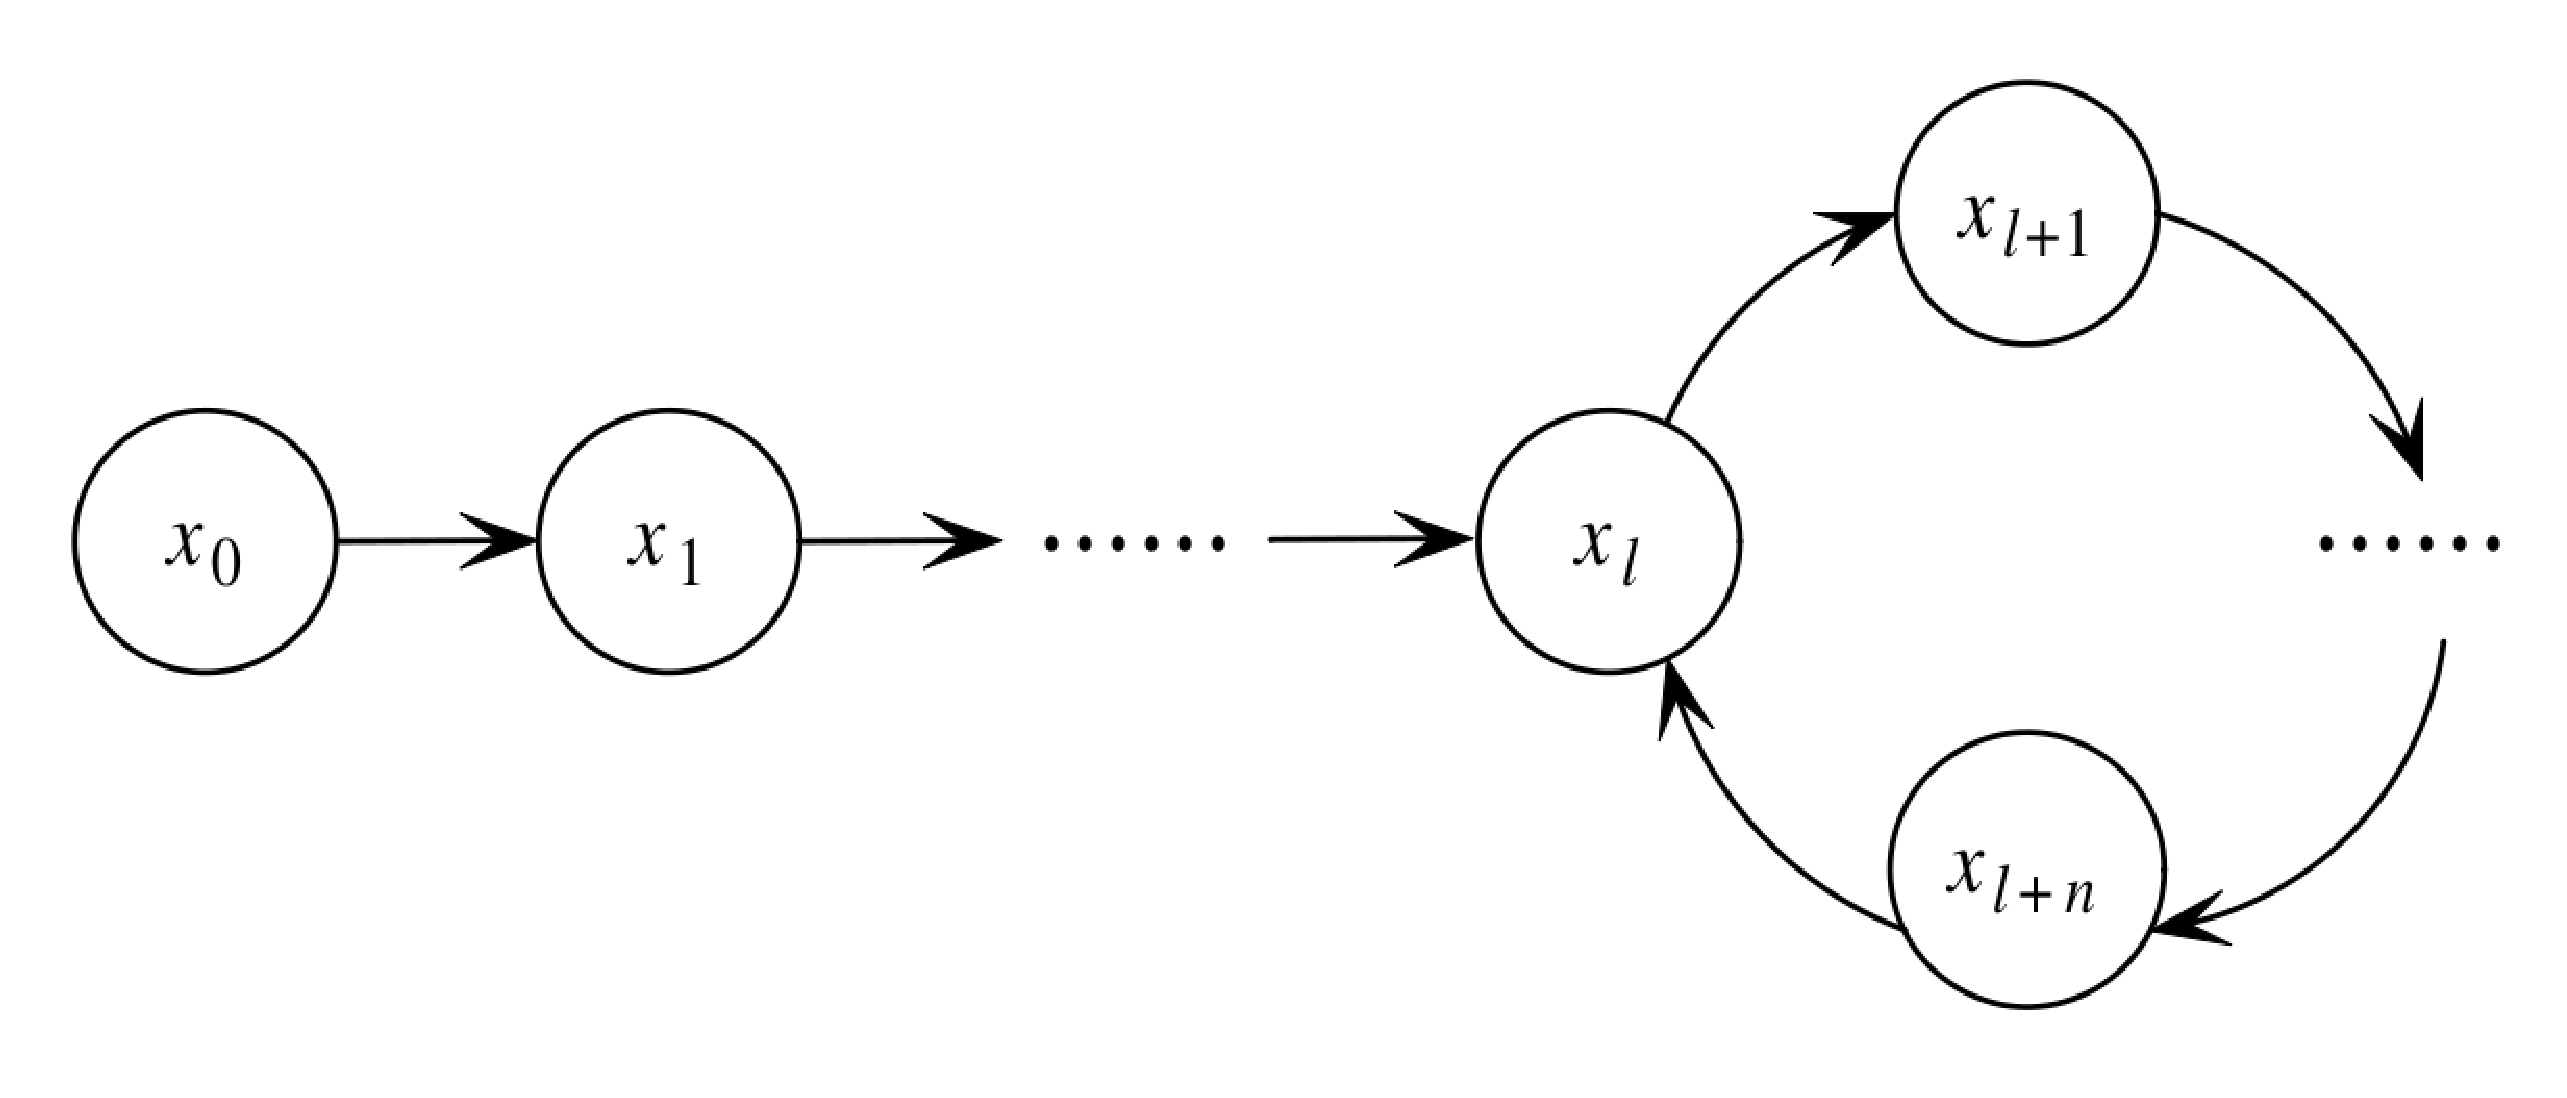
\includegraphics[scale=0.20]{images/pseudo_orbit.eps}
\caption{A pseudo orbit of a digital chaotic system}
\label{A pseudo orbit of a digital chaotic system}
\end{figure}


\begin{definition}%\cite{bahi102008}
A sequence $x = (x^{ 1} , ..., x^{n} )$ is said to be cyclic if a subset of successive terms is repeated from a given rank, until the end of $x$.
\end{definition}

This generator based on discrete chaotic iterations generated by two pseudorandom sequences ($m$ and $w$) has a long cycle length. If the cycle period of $m$ and $w$ are respectivelly $n_{m}$ and $n_{w}$, then in an ideal situation, the cycle period of the novel sequence is $n_{m} \times n_{w}\times 2$ (because $\bar{\bar{x}}=x$). Table \ref{The ideal cycle period} gives the ideal cycle period of various generators.

\begin{itemize}
\item $m$ ($n_{m}=2$): 12121212121212121212121212...

\item $w$ ($n_{w}=4$): 1 23 4 12 3 41 2 34 1 23 4 12 3 41 2 34 1 23 4...

\item $x$ ($n_{x}=2 \times 4 \times 2=16$): 0000(0) 1000(8) 1110(14) 1111(15) 0011(3) 0001(1) 1000(8) 1100(12) 1111(15) 0111(7) 0001(1) 0000(0) 1100(12) 1110(14) 0111(7) 0011(3) 0000(0) 1000(8) 1110(14) 1111(15) 0011(3) 0001(1) 1000(8) 1100(12) 1111(15) 0111(7) 0001(1) 0000(0) 1100(12) 1110(14) 0111(7) 0011(3)...

\end{itemize}


\begin{table}
\renewcommand{\arraystretch}{1.3}
\caption{Ideal cycle period}
\label{The ideal cycle period}
\centering
% \begin{tiny}
\begin{tabular}{|c|c|c|}\toprule\hline
\multicolumn{2}{|c|}{\textbf{PRNG}}&\textbf{Ideal cycle period}\\\hline
\multicolumn{2}{|c|}{\textbf{Logistic map}}& $\infty$\\\hline
\multicolumn{2}{|c|}{\textbf{XORshift}}&$2^{32}-1$ \\\hline
\multicolumn{2}{|c|}{\textbf{ISAAC}}& $2^{8295}$\\\hline
\multirow{4}*{\textbf{Old CI algorithms}}&\textbf{Logistic map 1+Logistic map 2}&$\infty$\\\cline{2-3}
&\textbf{XORshift+XORshift}&$2^{65}$\\\cline{2-3}
&\textbf{XORshift+ISAAC}&$2^{8328}$\\\cline{2-3}
&\textbf{ISAAC+ISAAC}&$2^{16591}$\\\hline
\bottomrule
\end{tabular}
% \end{tiny}
\end{table}


\section{New CI algorithms and examples}
\subsection{Presentation}
The CI generator (generator based on chaotic iterations) is designed by the following process. First of all, some chaotic iterations have to be done to generate a sequence $\left(x^n\right)_{n\in\mathds{N}} \in \left(\mathds{B}^\mathsf{N}\right)^\mathds{N}$ ($\mathsf{N} \in \mathds{N}^*, \mathsf{N} \geqslant 2$, $N$ is not necessarily equal to 32) of boolean vectors, which are the successive states of the iterated system. Some of these vectors will be randomly extracted and our pseudo-random bit flow will be constituted by their components. Such chaotic iterations are realized as follows. Initial state $x^0 \in \mathds{B}^\mathsf{N}$ is a boolean vector taken as a seed (see Section~\ref{algo seed}) and chaotic strategy $\left(S^n\right)_{n\in\mathds{N}}\in \llbracket 1, \mathsf{N} \rrbracket^\mathds{N}$ is
an irregular decimation of a random number sequence (Section~\ref{Chaotic strategy}). The iterate function $f$ is
the vectorial boolean negation:
$$f_0:(x_1,...,x_\mathsf{N}) \in \mathds{B}^\mathsf{N} \longmapsto (\overline{x_1},...,\overline{x_\mathsf{N}}) \in \mathds{B}^\mathsf{N}.$$
At each iteration, only the $S^i$-th component of state $x^n$ is updated, as follows: $x_i^n = x_i^{n-1}$ if $i \neq S^i$, else $x_i^n = \overline{x_i^{n-1}}$.
Finally, some $x^n$ are selected
by a sequence $m^n$ as the pseudo-random bit sequence of our generator.
$(m^n)_{n \in \mathds{N}} \in \mathcal{M}^\mathds{N}$ is computed from a PRNG, such as XORshift sequence $(y^n)_{n \in \mathds{N}} \in \llbracket 0, 2^{32}-1 \rrbracket$ (see Section~\ref{algo m}). So, the
generator returns the following values:\newline
\begin{small}
Bits:$$x_1^{m_0}x_2^{m_0}x_3^{m_0}\hdots x_\mathsf{N}^{m_0}x_1^{m_0+m_1}x_2^{m_0+m_1}\hdots x_\mathsf{N}^{m_0+m_1} x_1^{m_0+m_1+m_2}\hdots$$
or States:$$x^{m_0}x^{m_0+m_1}x^{m_0+m_1+m_2}\hdots$$
\end{small}


\subsection{The seed}
\label{algo seed}
The unpredictability of random sequences is established using
a random seed that is obtained by a physical source like timings of keystrokes.
Without the seed, the attacker must not be able to make any predictions about
the output bits, even when all details of the generator are known~\cite{Turan2008}.

The initial state of the system $x^0$ and the first term $y^0$ of the input PRNG are seeded either by
the current time in seconds since the Epoch, or by a number that the user inputs.
Different ways are possible. For example, let us denote by $t$ the decimal part of the current
time. So $x^0$ can be $t \text{ (mod $2^N$)}$ written in binary digits and $y^0 = t$.

\subsection{Sequence $m$ of returned states}
\label{algo m}
The output of the sequence $(y^n)$ is uniform in $\llbracket 0, 2^{32}-1 \rrbracket$. However, we do not want the output of $(m^n)$ to be uniform in $\llbracket 0, N \rrbracket$, because in this case, the returns of our generator will not be uniform in $\llbracket 0, 2^{N}-1 \rrbracket$, as it is illustrated in the following example. Let us suppose that $x^0=(0,0,0)$. Then $m^0 \in \llbracket 0, 3 \rrbracket$.
\begin{itemize}
\item If $m^0=0$, then no bit will change between the first and the second output of our new CI PRNG. Thus $x^1 = (0,0,0)$.
\item If $m^0=1$, then exactly one bit will change, which leads to three possible values for $x^1$, namely $(1,0,0)$, $(0,1,0)$, and $(0,0,1)$.
\item \emph{etc.}
\end{itemize}
As each value in $\llbracket 0, 2^3-1 \rrbracket$ must be returned with the same probability, then the values $(0,0,0)$, $(1,0,0)$, $(0,1,0)$, and $(0,0,1)$ must occur for $x^1$ with the same probability. Finally we see that, in this example, $m^0=1$ must be three times probable as $m^0=0$.
This leads to the following general definition for the probability of $m=i$:
\begin{equation}
P(m^n=i)=\frac{C^i_N}{2^N}
\end{equation}

Then, here is an example for the $(m^n)$ sequence with a selector function $g_1$
\begin{equation}
\label{Formula}
m^n = g_1(y^n)=
\left\{
\begin{array}{l}
0 \text{ if }0 \leqslant\frac{y^n}{2^{32}}<\frac{C^0_N}{2^N},\\
1 \text{ if }\frac{C^0_N}{2^N} \leqslant\frac{y^n}{2^{32}}<\sum_{i=0}^1\frac{C^i_N}{2^N},\\
2 \text{ if }\sum_{i=0}^1\frac{C^i_N}{2^N} \leqslant\frac{y^n}{2^{32}}<\sum_{i=0}^2\frac{C^i_N}{2^N},\\
\vdots~~~~~ ~~\vdots~~~ ~~~~\\
N \text{ if }\sum_{i=0}^{N-1}\frac{C^i_N}{2^N} \leqslant\frac{y^n}{2^{32}}<1.\\
\end{array}
\right.
\end{equation}

Let us notice, to conclude this subsection, that our new CI PRNG can use any reasonable function as selector. In this paper, $g_1()$ and $g_2()$ are adopted for demonstration purposes, where:
\begin{equation}
m^n = g_2(y^n)=
\left\{
\begin{array}{l}
N \text{ if }0 \leqslant\frac{y^n}{2^{32}}<\frac{C^0_N}{2^N},\\
N-1 \text{ if }\frac{C^0_N}{2^N} \leqslant\frac{y^n}{2^{32}}<\sum_{i=0}^1\frac{C^i_N}{2^N},\\
N-2 \text{ if }\sum_{i=0}^1\frac{C^i_N}{2^N} \leqslant\frac{y^n}{2^{32}}<\sum_{i=0}^2\frac{C^i_N}{2^N},\\
\vdots~~~~~ ~~\vdots~~~ ~~~~\\
0 \text{ if }\sum_{i=0}^{N-1}\frac{C^i_N}{2^N} \leqslant\frac{y^n}{2^{32}}<1.\\
\end{array}
\right.
\end{equation}

In this thesis, $g_1()$ is the selector function unless noted otherwise. And we will show later that both of $g_1()$ and $g_2()$ can pass all of the performed tests. 

%
%This definition has been chosen for the following reason:
%
%The probability $P$ of occurrences of any integer taken in $ \llbracket 0;\mathsf{2^N}-1 \rrbracket$ is $\frac{1}{2^N}$. A string of $N$ binary digits is used to represent this integer; changing $m$ bits of this string will lead to $C_N^m$ different integers.
%
%
%$m^n$ indicates the changing bits between two adjacent output values.
%
%
%If the CI generator generate numbers, each approximately uniformly selected from the set
%$\llbracket 0;\mathsf{2^N}-1 \rrbracket$, the probability
%distribution $P_m$ of $m$ from the XORshift is equal to $\frac{C_N^m}{2^N}$.
%


%$y^0 \in \llbracket 0;2^{32}-1 \rrbracket$ be an integer deduced as a seed too (see Section \ref{algo seed}).
% As shown in Figure~\ref{}, It means that the velue of y_{n+1} can be selected as any values.
% Color histogram. In order to appear random, the color histograms of the encrypted image should be uniform
% distributed in all three color components (RGB). Figs. 6 and 7 show the histograms of RGB colors for the
% original (Fig. 5(a)) and the encrypted images (Fig. 5(b)), respectively. It can be observed that a flat color his-
% togram is resulted from the encrypted image using our scheme. Its uniformity is further justified by the chi-
% square test [14]
In order to evaluate our proposed method and compare its statistical properties with various other methods, the density histogram and intensity map of adjacent output have been computed. The length of $x$ is $N = 4$ bits, and the initial conditions and control
parameters are the same. A large number of
sampled values are simulated ($10^6$ samples). 
%As shown in Figure~\ref{Histogram and intensity map}, it means that the number of adjacent output exists within the sequence. 
Figure~\ref{Histogram1} and Figure~\ref{Histogram2} shows the intensity map for $m^n=g_1(y^n)$ and $m^n=g_2(y^n)$.
In order to appear random, the histogram should be uniformly distributed in all areas. 
It can be observed that uniform histograms and flat color intensity maps are obtained when using our schemes. 
Another illustration of this fact is given by Figure~\ref{Histogram3}, whereas its uniformity is further justified by the tests presented in Section \ref{Results of NISTfor new CI}.
% and for $m^n=y^n~mod~N$ () respectively.  


\begin{figure}[!t]
\centering
\subfigure [The histogram of adjacent output distribution $m^n = g_1(y^n)$]{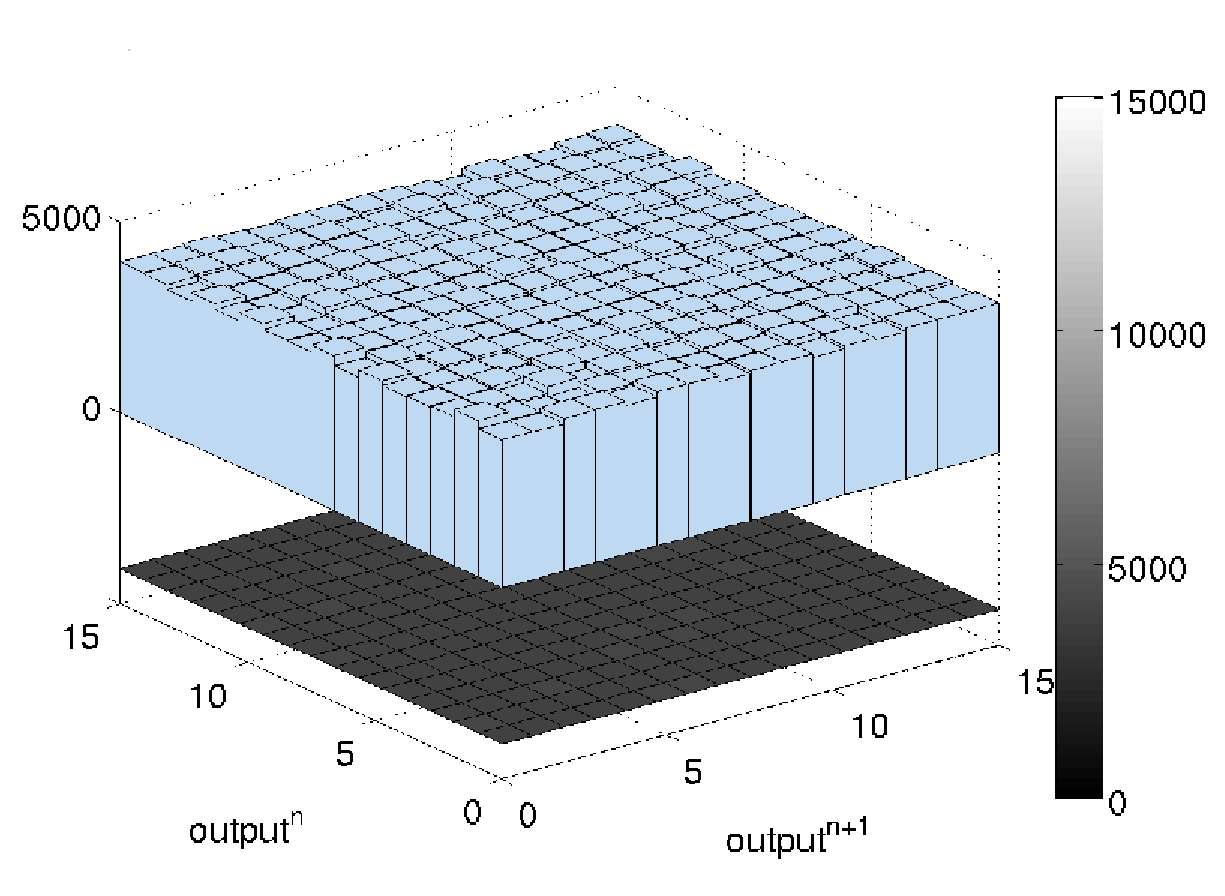
\includegraphics[scale=0.4]{images/f(y).eps}
\label{Histogram1}} \hspace{0.4cm}
\subfigure [The histogram of adjacent output distribution $m^n = g_2(y^n)$]{\includegraphics[scale=0.3]{images/f2(y).eps}
\label{Histogram2}} \hspace{0.4cm}
\subfigure [The histogram of adjacent output distribution $m^n = y^n ~ mod ~ 4$]{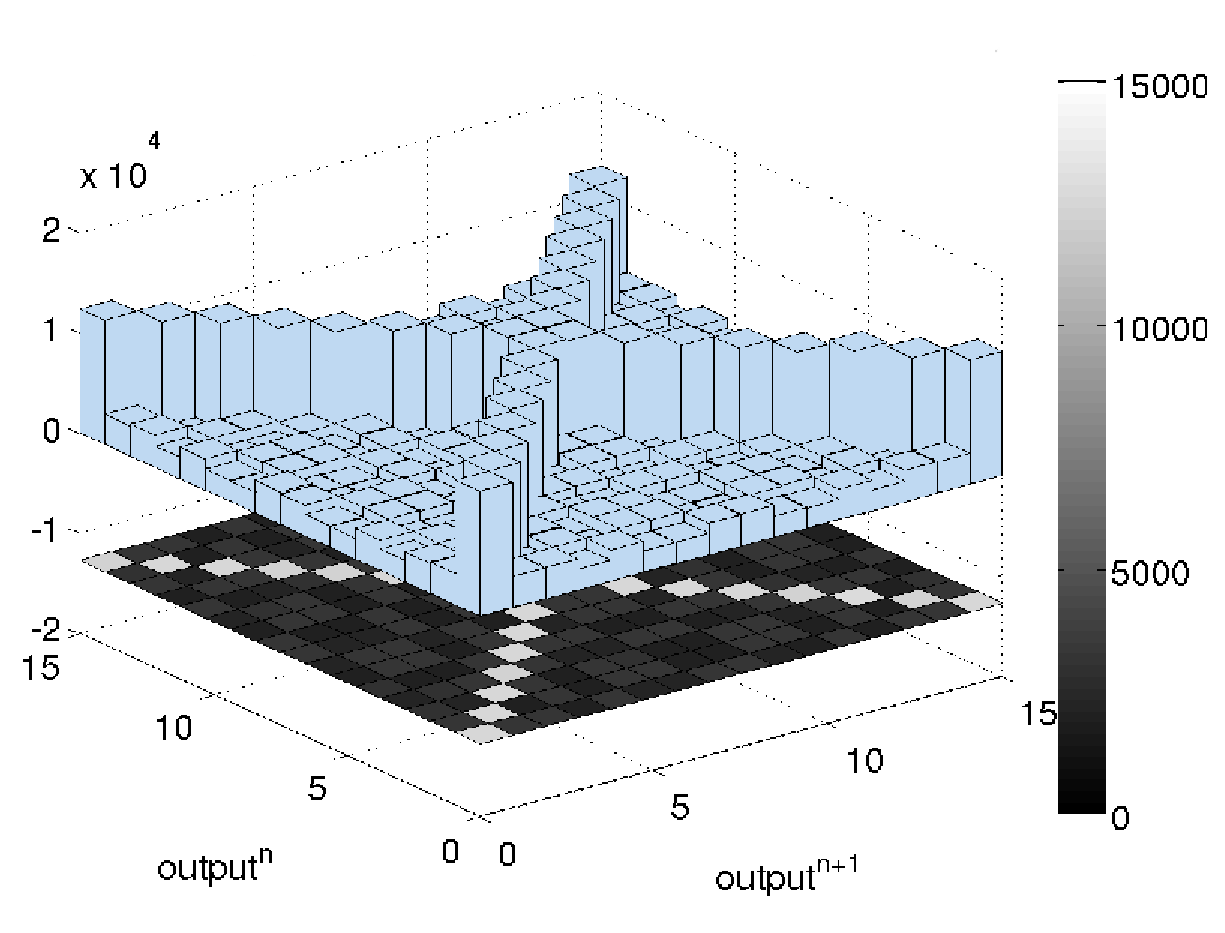
\includegraphics[scale=0.4]{images/y.eps}%
\label{Histogram3}} \hspace{0.4cm}
\caption{Histogram and intensity maps}
\label{Histogram and intensity map1}
\end{figure}


\subsection{Chaotic strategy}
\label{Chaotic strategy}
The chaotic strategy $(S^k) \in \llbracket 1, N \rrbracket^\mathds{N}$ is generated from a second XORshift sequence $(b^k) \in \llbracket 1, N \rrbracket^\mathds{N}$. The only difference between the sequences $S$ and $b$ is that some terms of $b$ are discarded, in such a way that $\forall k \in \mathds{N}, (S^{M^k}, S^{M^k+1}, \hdots, S^{M^{k+1}-1})$ does not contain any given integer twice, where $M^k = \sum_{i=0}^k m^i$. Therefore, no bit will change more than once between two successive outputs of our PRNG, increasing the speed of the former generator by doing so. $S$ is said to be ``an irregular decimation'' of $b$. This decimation can be obtained by the following process.

Let $(d^1,d^2,\dots,d^N)\in \{0,1\}^N$ be a mark sequence, such that whenever $\sum_{i=1}^N d^i = m^k$,
then $\forall i, d_i=0$ ($\forall k$, the sequence is reset when $d$ contains $m^k$ times the number 1). This mark sequence will control the XORshift sequence $b$ as follows:
\begin{itemize}
\item if $d^{b^j} \neq 1$, then $S^k=b^j$, $d^{b^j} = 1$, and $k = k+1$,
\item if $d^{b^j}=1$, then $b^j$ is discarded.
\end{itemize}
For example, if $b = 142\underline{2}334 1421\underline{1}\underline{2}\underline{2}34...$ and $m = 4341...$, then $S=1423~341~4123~4...$ However, if we do not use the mark sequence, then one position may change more than once and the balance property will not be checked, due to the fact that $\bar{\bar{x}}=x$. As an example, for $b$ and $m$ as in the previous example, $S=1422~334~1421~1...$ and $S=14~4~42~1...$ lead to the same output (because switching the same bit twice leads to the same state).

 
To check the balance property, a set of 500
sequences are generated with and without decimation, each
sequence containing $10^6$ bits. Figure~\ref{nmark} shows the
percentages of differences between zeros and ones, and presents a better balance property for the sequences with decimation. This claim will be verified in the tests section (Section \ref{Results of NISTfor new CI}). 


Another example is given in Table~\ref{table application example}, in which $r$ means ``reset'' and the integers which are underlined in sequence $b$ are discarded.
%A simple example illustrates the behavior of this structure.\\
%$m$ : 0,~~~~~~~~~~~~~~~~~~~~~~~~~~~~~~~~~~~~~~~~~~~~~~~~~~~~~~~~~~~4,~~~~~~~~~~~~~~~~~~~~~~~~~~~~~2,\\
%$d$ : r(1,0,0,0),(1,0,0,1),(1,1,0,1),(1,1,1,1),r(0,0,1,0),(0,0,1,1),r \\
%$b$ : ~~~ 1,~~~~~~~~~~~ 4,~~~~~~~~~~~~ 2,~~~~ \underline{2},~~~~ 3,~~~~~~~~~~~~~~3,~~~~~~~~~~~~~ 4,~~~~~~~~~~~~~~~~\\
%$S$ : ~~~1,~~~~~~~~~~~ 4,~~~~~~~~~~~~ 2,~~~~~~~~~~~~ 3,~~~~~~~~~~~~~~3,~~~~~~~~~~~~~ 4,~~~~~~~~~~~~~~~~
%
%Here r means reset, the underlined numbers in the sequence $b_j$ are discarded. In brief, the
%sequence $S$ is an irregular decimation of $b$ by the mark sequence.






\begin{figure}
\centering
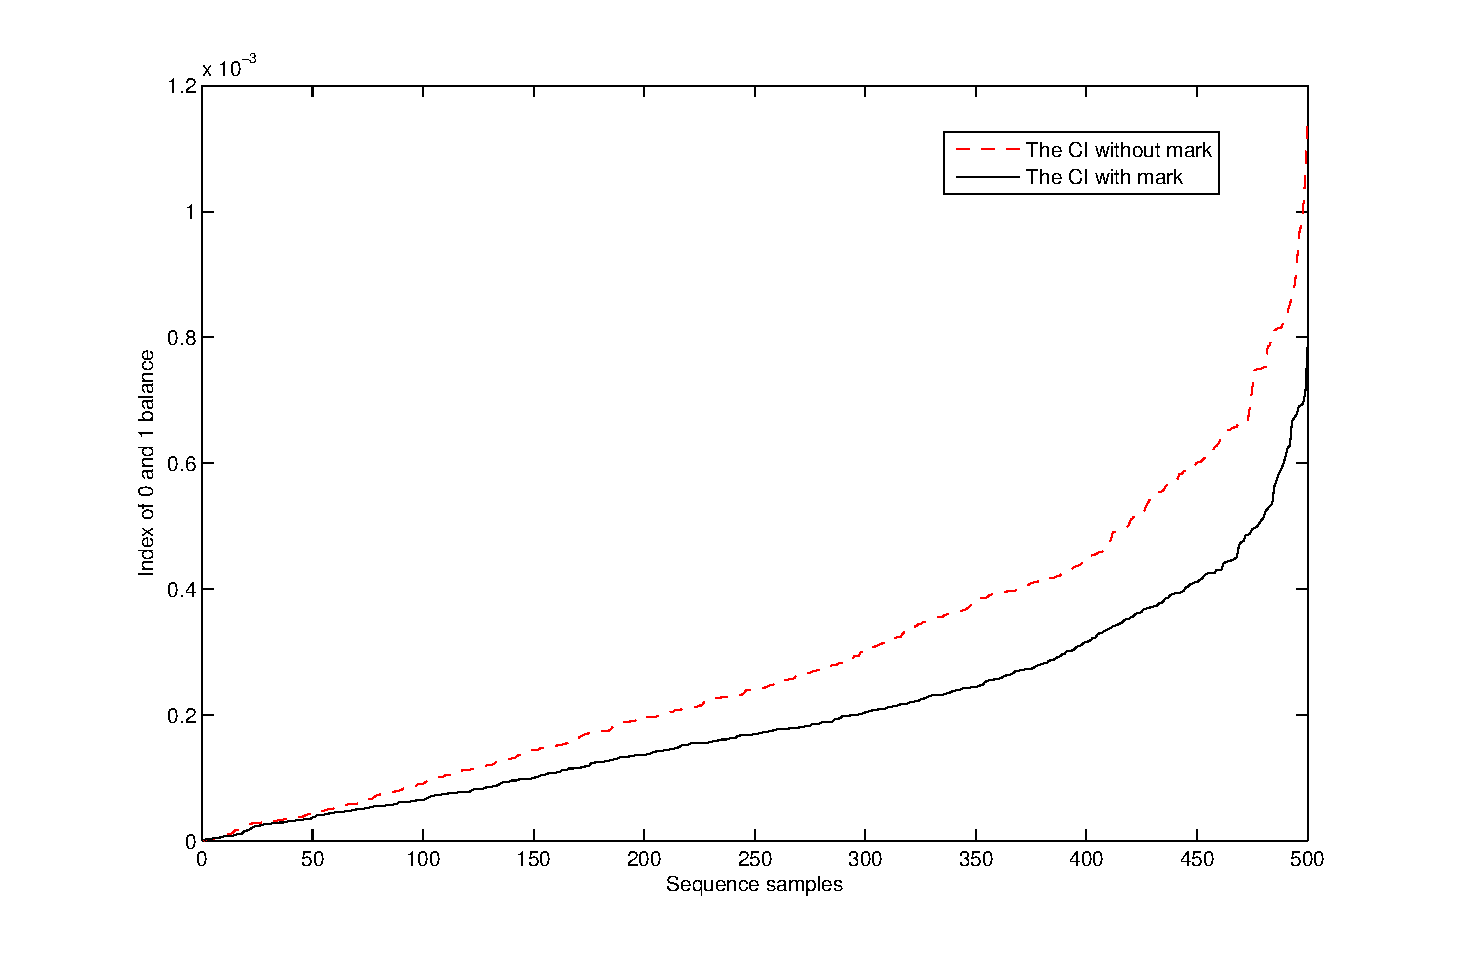
\includegraphics[width=3.85in]{images/nmark.eps}
\DeclareGraphicsExtensions.
\caption{Balance property}
\label{nmark}
\end{figure}

\subsection{New CI(XORshift, XORshift) Algorithm}

The basic design procedure of the novel generator is summed up in Algorithm~\ref{Chaotic iteration1}.
The internal state is $x$, the output state is $r$. $a$ and $b$ are those computed by the two input
PRNGs. The value $g_1(a)$ is an integer, defined as in Equation~\ref{Formula}. Lastly, $\mathsf{N}$ is a constant defined by the user.
\begin{algorithm}
\textbf{Input:} the internal state $x$ ($\mathsf{N}$ bits)\\
\textbf{Output:} a state $r$ of $\mathsf{N}$ bits
\begin{algorithmic}[1]
\FOR{$i=0,\dots,N$}
{
\STATE$d_i\leftarrow{0}$\;
}
\ENDFOR
\STATE$a\leftarrow{PRNG1()}$\;
\STATE$m\leftarrow{f(a)}$\;
\STATE$k\leftarrow{m}$\;
\WHILE{$i=0,\dots,k$}

\STATE$b\leftarrow{PRNG2()~mod~\mathsf{N}}$\;
\STATE$S\leftarrow{b}$\;
    \IF{$d_S=0$}
    {
\STATE      $x_S\leftarrow{ \overline{x_S}}$\;
\STATE      $d_S\leftarrow{1}$\;
    
    }
    \ELSIF{$d_S=1$}
    {
\STATE      $k\leftarrow{ k+1}$\;
    }\ENDIF
\ENDWHILE
$r\leftarrow{x}$\;
return $r$\;
\medskip
\caption{An arbitrary round of the new CI generator}
\label{Chaotic iteration1}
\end{algorithmic}
\end{algorithm}

% 
% \begin{algorithm}
% \SetAlgoLined
% \KwIn{the internal state $x$ ($\mathsf{N}$ bits)}
% \KwOut{a state $r$ of $\mathsf{N}$ bits}
% \For{$i=0,\dots,N$}
% {
% $d_i\leftarrow{0}$\;
% }
% $a\leftarrow{XORshift1()}$\;
% $m\leftarrow{g_1(a)}$\;
% $k\leftarrow{m}$\;
% \For{$i=0,\dots,k$}
% {
% $b\leftarrow{XORshift2()~mod~\mathsf{N}}$\;
% $S\leftarrow{b}$\;
% \If{$d_S=0$}
% {
% $x_S\leftarrow{ \overline{x_S}}$\;
% $d_S\leftarrow{1}$\;
% }
% \ElseIf{$d_S=1$}
% {
% $k\leftarrow{ k+1}$\;
% }
% }
% $r\leftarrow{x}$\;
% return $r$\;
% \medskip
% \caption{An arbitrary round of the new CI(XORshift,XORshift) generator}
% \label{Chaotic iteration1}
% \end{algorithm}

As a comparison, the basic design procedure of the old generator is recalled in Algorithm~\ref{Chaotic iteration2} ($a$ and $b$ are computed by two input PRNGs, $\mathsf{N}$ and $c\geqslant 3\mathsf{N}$ are constants defined by the user). See Subsection~\ref{Old CI algorithms and examples} for further information.

% \begin{algorithm}
% \SetAlgoLined
% \KwIn{the internal state $x$ ($\mathsf{N}$ bits)}
% \KwOut{a state $r$ of $\mathsf{N}$ bits}
% $a\leftarrow{Logistic map1()}$\;
% \If{$a>0.5$}
% {
% $d\leftarrow 1$
% }
% \Else
% {
% $d\leftarrow 0$
% }
% 
% $m\leftarrow{d+c}$\;
% \For{$i=0,\dots,m$}
% {
% $b\leftarrow{Logistic map2()}$\;
% $S\leftarrow{100000b~mod~\mathsf{N}}$\;
% $x_S\leftarrow{ \overline{x_S}}$\;
% }
% $r\leftarrow{x}$\;
% return $r$\;
% \medskip
% \caption{An arbitrary round of the old CI PRNG}
% \label{Chaotic iteration2}
% \end{algorithm}
\begin{algorithm}
\textbf{Input:} the internal state $x$ (an array of $\mathsf{N}$ 1-bit words)\\
\textbf{Output:} an array $r$ of $\mathsf{N}$ 1-bit words
\begin{algorithmic}[1]

\STATE$a\leftarrow{PRNG1()}$;
\STATE$m\leftarrow{a~mod~2+c}$;
\WHILE{$i=0,\dots,m$}
\STATE$b\leftarrow{PRNG2()}$;
\STATE$S\leftarrow{b~mod~\mathsf{N}}$;
\STATE$x_S\leftarrow{ \overline{x_S}}$;
\ENDWHILE
\STATE$r\leftarrow{x}$;
\STATE return $r$;
\medskip
\caption{An arbitrary round of the old CI generator}
\label{Chaotic iteration2}
\end{algorithmic}
\end{algorithm}


\subsection{Illustrative Example}

In this example, $\mathsf{N} = 4$ is chosen for easy understanding and the input PRNG is XORshift PRNG.
As stated before, the initial state of the system $x^0$ can be seeded by the decimal part $t$ of the current time.
For example, if the current time in seconds since the Epoch is 1237632934.484088,
so $t = 484088$, then $x^0 = t \text{ ($mod$ 16)}$ in binary digits, \emph{i.e.}, $x^0 = ( 0, 1, 0, 0)$.

To compute $m$ sequence, Equation~\ref{Formula} can be adapted to this example as follows:
\begin{equation}
\label{m1 fuction}
m^n=g_1(y^n)=
\left\{
\begin{array}{llccccc}
0 & \text{ if }&0 &\leqslant&\frac{y^n}{2^{32}}&<&\frac{1}{16},\\
1 & \text{ if }&\frac{1}{16} &\leqslant&\frac{y^n}{2^{32}}&<&\frac{5}{16} ,\\
2 & \text{ if }&\frac{5}{16} &\leqslant&\frac{y^n}{2^{32}}&<&\frac{11}{16},\\
3 & \text{ if }&\frac{11}{16} &\leqslant&\frac{y^n}{2^{32}}&<&\frac{15}{16},\\
4 & \text{ if }&\frac{15}{16} &\leqslant&\frac{y^n}{2^{32}}&<&1,\\
\end{array}
\right.
\end{equation}

\noindent where $y$ is generated by XORshift seeded with the current time. We can see that the probabilities of occurrences of $m=0$, $m=1$, $m=2$, $m=3$, $m=4$, are $\frac{1}{16}$, $\frac{4}{16}$, $\frac{6}{16}$, $\frac{4}{16}$, $\frac{1}{16}$, respectively. This $m$ determines what will be the next output $x$. For instance,
\begin{itemize}
\item If $m=0$, the following $x$ will be $( 0, 1, 0, 0)$.
\item If $m=1$, the following $x$ can be $( 1, 1, 0, 0)$, $( 0, 0, 0, 0)$, $( 0, 1, 1, 0)$, or $( 0, 1, 0, 1)$.
\item If $m=2$, the following $x$ can be $( 1, 0, 0, 0)$, $( 1, 1, 1, 0)$, $( 1, 1, 0, 1)$, $( 0, 0, 1, 0)$, $( 0, 0, 0, 1)$, or $( 0, 1, 1, 1)$.
\item If $m=3$, the following $x$ can be $( 0, 0, 1, 1)$, $( 1, 1, 1, 1)$, $( 1, 0, 0, 1)$, or $( 1, 0, 1, 0)$.
\item If $m=4$, the following $x$ will be $( 1, 0, 1, 1)$.
\end{itemize}

In this simulation, $m = 0, 4, 2, 2, 3, 4, 1, 1, 2, 3, 0, 1, 4,...$ Additionally, $b$ is computed with a XORshift generator too, but with another seed. We have found $b = 1, 4, 2, 2, 3, 3, 4, 1, 1, 4, 3, 2, 1,...$

Chaotic iterations are made with initial state $x^0$, vectorial logical negation $f_0$, and
strategy $S$. The result is presented in Table~\ref{table application example}. Let us recall that sequence $m$ gives the states $x^n$ to return, which are here $x^0, x^{0+4}, x^{0+4+2}, \hdots$ So, in this example, the output of the generator is: 10100111101111110011... or 4,4,11,8,1...




\begin{table*}[!t]
%\renewcommand{\arraystretch}{1.3}
\centering
\begin{tabular}{|c|c@{}c|c@{}c@{}c@{}c@{}c@{}c|c@{}c@{}c|c@{}c@{}c@{}c|}
\hline
$m$ &0 & &4 & & & & & &2& &&2&&  &  \\ \hline
$k$ &0 & &4 & & &$+1$ & & &2& &&2&$+1$&  &  \\ \hline
$b$  &  & &1 &4&2&\underline{2}       &3& &3&4&&1&\underline{1}      &4&\\ \hline
$d$  &r  & &r~$\left(\begin{array}{c}1\\0\\0\\0\end{array}\right)$ & $\left(\begin{array}{c}1\\0\\0\\1\end{array}\right)$ & $\left(\begin{array}{c}1\\1\\0\\1\end{array}\right)$ & & $\left(\begin{array}{c}1\\1\\1\\1\end{array}\right)$ && r~$\left(\begin{array}{c}0\\0\\1\\0\end{array}\right)$ &$\left(\begin{array}{c}0\\0\\1\\1\end{array}\right)$ &&r~$\left(\begin{array}{c}1\\0\\0\\0\end{array}\right)$ & &$\left(\begin{array}{c}1\\0\\0\\1\end{array}\right)$  &  \\ \hline
$S$  &  & &1 &4&2&        &3& &3&4&&1& &4 &  \\ \hline
$x^{0}$ &  &$x^{0}$ & & &  
&  & &$x^{4}$ & & &   
$x^{6}$& & &&$x^{8}$  \\
%1ere ligne
0 & &0 &$\xrightarrow{1} 1$ & &
 & &   &1   & & &
1 &$\xrightarrow{1} 0$ & & & 0\\
%2eme ligne
1 &  &1 &   &   &
$\xrightarrow{2} 0$ & & &0 & & &
0 & &  &&0\\
%3eme ligne
0 & &0 & & &
 & &$\xrightarrow{3} 1$ &1 &$\xrightarrow{3} 0$ & &
0 &   & & &0  \\
% 4eme ligne
0 & &0  & &$\xrightarrow{4} 1$ &
 & & &1 & &$\xrightarrow{4} 0$ &
0 & & &$\xrightarrow{4} 1$&1 \\
\hline
\end{tabular}\\
\vspace{0.5cm}
Binary Output: $x_1^{0}x_2^{0}x_3^{0}x_4^{0}x_1^{4}x_2^{4}x_3^{4}x_4^{4}x_1^{6}x_2^{6}... = 0100101110000001...$\\
Integer Output:
$x^{0},x^{4},x^{6},x^{8}... = 4,11,8,1...$
\caption{Example of New CI(XORshift,XORshift) generation}
\label{table application example}
\end{table*}







% 
% \section{Chaotic iterations as pseudo-random generator}
% \subsection{Presentation}
% 
% The CI generator is designed by the following process \cite{wang2009,wbg10:ip}. 
% 
% Chaotic iterations are done to generate a sequence $\left(x^n\right)_{n\in\mathds{N}} \in \left(\mathds{B}^\mathsf{N}\right)^\mathds{N}$ ($\mathsf{N} \in \mathds{N}^*, \mathsf{N} \geqslant 2$) of boolean vectors, which are the successive states of the iterated system. Some of these vectors are randomly extracted and the pseudo-random bit flow is constituted by their components. These chaotic iterations are realized as follows. 
% 
% Initial state $x^0 \in \mathds{B}^\mathsf{N}$ is a boolean vector taken as a seed (see Section~\ref{algo seed}) and chaotic strategy $\left(S^n\right)_{n\in\mathds{N}}\in \llbracket 1, \mathsf{N} \rrbracket^\mathds{N}$ is defined with a XORshift sequence (Old CI generator \cite{wang2009}) or an irregular decimation of it (New CI generatot \cite{wbg10:ip}), as it is explained in Section~\ref{Chaotic strategy}). Lastly, the iterate function $f$ is the vectorial boolean negation.
% 
% More precisely, at each iteration, only $S^i$-th component of state $x^n$ is updated as follows
% \begin{equation}
% x_i^n = \left\{\begin{array}{ll}x_i^{n-1} & \text{if } i \neq S^i, \\ \\ \overline{x_i^{n-1}} & \text{if } i = S^i. \\\end{array}\right.
% \end{equation}
% Then, let $\mathcal{M}$ be a finite subset of $\mathds{N}^*$. Some $x^n$ are selected by a sequence $m^n$ as the pseudo-random bit sequence of our generator. The sequence $(m^n)_{n \in \mathds{N}} \in \mathcal{M}^\mathds{N}$ is computed from XORshift (or from a decimation of it, in case of the new CI generator). So, the generator returns the following values:
% \begin{itemize}
% \item the components of $x^{m^0}$,
% \item following by the components of $x^{m^0+m^1}$,
% \item following by the components of $x^{m^0+m^1+m^2}$,
% \item \emph{etc.}
% \end{itemize}
% In other words, the generator returns the following bits:\newline
% \begin{small}
% $$x_1^{m_0}x_2^{m_0}x_3^{m_0}\hdots x_\mathsf{N}^{m_0}x_1^{m_0+m_1}x_2^{m_0+m_1}\hdots x_\mathsf{N}^{m_0+m_1} x_1^{m_0+m_1+m_2}x_2^{m_0+m_1+m_2}\hdots$$
% \end{small}
% 
% 
% 
% \subsection{The seed}
% \label{algo seed}
% 
% The initial state of the system $x^0$ and the first term $y^0$ of the XORshift are seeded either by the current time in seconds since the Epoch, or by a number that the user inputs, as it is usually the case for every PRNG.
% 
% \subsection{Sequence $m$ of returned states}
% \label{algo m}
% 
% The output of a sequence $(y^n)$ produced by a XORshift generator is uniform in $\llbracket 0, 2^{32}-1 \rrbracket$. However, we do not want the output of $(m^n)$ to be uniform in $\llbracket 0, N \rrbracket$, because in this case, the returns of our generator will not be uniform in $\llbracket 0, 2^{N}-1 \rrbracket$, as it is illustrated in the following example. Let us suppose that $x^0=(0,0,0)$. Then $m^0 \in \llbracket 0, 3 \rrbracket$.
% \begin{itemize}
% \item If $m^0=0$, then no bit will change between the first and the second output of our PRNG. Thus $x^1 = (0,0,0)$.
% \item If $m^0=1$, then exactly one bit will change, which leads to three possible values for $x^1$, namely $(1,0,0)$, $(0,1,0)$, and $(0,0,1)$.
% \item \emph{etc.}
% \end{itemize}
% As each value in $\llbracket 0, 2^3-1 \rrbracket$ must be returned with the same probability, then the values $(0,0,0)$, $(1,0,0)$, $(0,1,0)$ and $(0,0,1)$ must occur for $x^1$ with the same probability. Finally we see that, in this example, $m^0=1$ must be three times more probable than $m^0=0$.
% This leads to the following general definition for $m$:
% \begin{equation}
% \label{Formula}
% m^n = f(y^n)=
% \left\{
% \begin{array}{l}
% 0 \text{ if }0				\leqslant\frac{y^n}{2^{32}}<\frac{C^0_N}{2^N},\\
% 1 \text{ if }\frac{C^0_N}{2^N}		\leqslant\frac{y^n}{2^{32}}<\sum_{i=0}^1\frac{C^i_N}{2^N},\\
% 2 \text{ if }\sum_{i=0}^1\frac{C^i_N}{2^N}	\leqslant\frac{y^n}{2^{32}}<\sum_{i=0}^2\frac{C^i_N}{2^N},\\
% \vdots~~~~~					~~\vdots~~~		    ~~~~\\
% N \text{ if }\sum_{i=0}^{N-1}\frac{C^i_N}{2^N}	\leqslant\frac{y^n}{2^{32}}<1.\\
% \end{array}
% \right.
% \end{equation}
% %
% %This definition has been chosen for the following reason: 
% %
% %The probability $P$ of occurrences of any integer taken in $ \llbracket 0;\mathsf{2^N}-1 \rrbracket$ is $\frac{1}{2^N}$. A string of $N$ binary digits is used to represent this integer; changing $m$ bits of this string will lead to $C_N^m$ different integers.
% %
% %
% %$m^n$ indicates the changing bits between two adjacent output values.
% %
% %
% %If the CI generator generate numbers, each approximately uniformly selected from the set 
% %$\llbracket 0;\mathsf{2^N}-1 \rrbracket$, the probability 
% %distribution $P_m$ of $m$ from the XORshift is equal to $\frac{C_N^m}{2^N}$.
% %
% 
% 
% %$y^0 \in \llbracket 0;2^{32}-1 \rrbracket$ be an integer deduced as a seed too (see Section \ref{algo seed}).
% 
% 
% \subsection{Chaotic strategy}
% \label{Chaotic strategy}
% 
% The chaotic strategy $(S^k) \in \llbracket 1, N \rrbracket^\mathds{N}$ is generated from a second XORshift sequence $(b^k) \in \llbracket 1, N \rrbracket^\mathds{N}$. In the Old CI generator, $S=b$. In the New CI generator, the sole difference between the sequences $S$ and $b$ is that some terms of $b$ are discarded, in such a way that: $\forall k \in \mathds{N}, (S^{M^k}, S^{M^k+1}, \hdots, S^{M^{k+1}-1})$ does not contain a same integer twice, where $M^k = \sum_{i=0}^k m^i$. Therefore, in New CI generator, no bit will change more than once between two successive outputs of our PRNG, increasing the speed of the former generator by doing so. $S$ is said to be ``an irregular decimation'' of $b$. This decimation can be obtained by the following process.
% 
% Let $(d^1,d^2,\dots,d^N)\in \{0,1\}^N$ be a mark sequence, such that whenever $\sum_{i=1}^N d^i = m^k$, 
% then $\forall i, d_i=0$ ($\forall k$, the sequence is reset when $d$ contains $m^k$ times the number 1). This mark sequence will control the XORshift sequence $b$ as follows:
% \begin{itemize}
% \item if $d^{b^j} \neq 1$, then $S^k=b^j$, $d^{b^j} = 1$, and $k = k+1$,
% \item if $d^{b^j}=1$, then $b^j$ is discarded.
% \end{itemize}
% For example, if $b = 142\underline{2}334 142\underline{1}\underline{1}\underline{2}\underline{2}34...$ and $m = 4241...$, then $S=1423~34~1423~4...$ Another example is given in Table~\ref{table application example}, in which $r$ means ``reset'' and the integers which are underlined in sequence $b$ are discarded.
% 
% 
% 
% %\subsection{Old CI pseudo-random sequence}
% %\label{The generation of pseudo-random sequence}
% 
% %The design of the PRNG based on discrete chaotic iterations is proposed in this section, while its performance is evaluated in the next sections.
% %The old CI generator is designed by the following process.
% %Let $\mathsf{N} \in \mathds{N}^*, \mathsf{N} \geqslant 2$. Some chaotic iterations are done, which generate a sequence $\left(x^n\right)_{n\in\mathds{N}} \in \left(\mathds{B}^\mathsf{N}\right)^\mathds{N}$ of boolean vectors: the successive states of the iterated system. Some of these vectors are chaotically extracted and their components constitute our pseudo-random bit flow.
% %Chaotic iterations are realized as follows: initial state\linebreak $x^0 \in \mathds{B}^\mathsf{N}$ is a boolean vector taken as a seed and chaotic strategy $\left(S^n\right)_{n\in\mathds{N}}\in \llbracket 1, \mathsf{N} \rrbracket^\mathds{N}$ is constructed with XORshift. Lastly, iterate function $f$ is the vectorial boolean negation
% %$$f_0:(x_1,...,x_\mathsf{N}) \in \mathds{B}^\mathsf{N} \longmapsto (\overline{x_1},...,\overline{x_\mathsf{N}}) \in \mathds{B}^\mathsf{N}.$$
% 
% 
% 
% 
% 
% 
% \section{CI(XORshift, XORshift) algorithms and examples}
% 
% \subsection{Algorithms}
% 
% The basic design procedure of the old generator is recalled in Algorithm~\ref{Chaotic iteration2} ($a$ and $b$ are computed by XORshift generators, $\mathsf{N}$ and $c\geqslant 3\mathsf{N}$ are constants defined by the user). 
% Algorithm~\ref{Chaotic iteration1} summarizes the basic design procedure of the new generator. The internal state is $x$, the output state is $r$. $a$ and $b$ are those computed by the two XORshift generators. The value $f(a)$ is an integer, defined as in Equation~\ref{Formula}. Lastly, $\mathsf{N}$ is a constant defined by the user.
% 
% 
% \begin{algorithm}
% \textbf{Input:} the internal state $x$ (an array of $\mathsf{N}$ 1-bit words)\\
% \textbf{Output:} an array $r$ of $\mathsf{N}$ 1-bit words
% \begin{algorithmic}[1]
% 
% \STATE$a\leftarrow{XORshift1()}$;
% \STATE$m\leftarrow{a~mod~2+c}$;
% \WHILE{$i=0,\dots,m$}
% \STATE$b\leftarrow{XORshift2()}$;
% \STATE$S\leftarrow{b~mod~\mathsf{N}}$;
% \STATE$x_S\leftarrow{ \overline{x_S}}$;
% \ENDWHILE
% \STATE$r\leftarrow{x}$;
% \STATE return $r$;
% \medskip
% \caption{An arbitrary round of the old CI(XORshift,XORshift) generator}
% \label{Chaotic iteration2}
% \end{algorithmic}
% \end{algorithm}
% 
% 
% \subsection{Old CI(XORshift,XORshift) example}
% 
% 
% 
% In this example, $\mathsf{N} = 5$ and $\mathcal{M} = \{\text{4,5}\}$ are adopted for easy understanding.
% The initial state of the system $x^0$ can be seeded by the decimal part of the current time. For example, the current time in seconds since the Epoch is 1237632934.484084, so $t = 484084$. $x^0 = t \text{ (mod 32)}$ in binary digits, then $x^0 = (1, 0, 1, 0, 0)$. $m$ and $S$ can now be computed from two XORshift PRNGs:
% 
% $m$ = 4, 5, 4, 4, 4, 4, 5, 5, 5, 5, 4, 5, 4,...
% 
% $S$ = 2, 4, 2, 2, 5, 1, 1, 5, 5, 3, 2, 3, 3,...
% 
% Chaotic iterations are done with initial state $x^0$, vectorial logical negation $f_0$ and strategy $S$. The result is presented in Table \ref{Table:old CI}. Let us recall that sequence $m$ gives the states $x^n$ to return: $x^4, x^{4+5}, x^{4+5+4}, \hdots$
% 
% 
% \begin{tiny}
% \begin{table}[!t]
% \renewcommand{\arraystretch}{1.3}
% \caption{Application example (Old CI generator)}
% \label{Table:old CI}
% \centering
% \begin{tabular}{c|c@{}c@{}c@{}c@{}c|c@{}c@{}c@{}c@{}c@{}c|c@{}c@{}c@{}c@{}c@{}c}
% \hline\hline
% $m:$ & & & 4 & & & & & 5 & & & & & & 4 & & & \\ \hline
% $S$ & 2 & 4 & 2 & 2 & & 5 & 1 & 1 & 5 & 5 & & 3 & 2 & 3 & 3 & & \\ \hline
% $x^{0}$ & & & & & $x^{4}$ & & & & & & $x^{9}$ & & & & & $x^{13}$ & \\
% %1ere ligne
% 1 & & & & &
% 1 & & $\xrightarrow{1} 0$ & $\xrightarrow{1} 1$ & & &
% 1 & & & & &
% 1 & \\
% %2eme ligne
% 0 & $\xrightarrow{2} 1$ & & $\xrightarrow{2} 0$ & $\xrightarrow{2} 1$ &
% 1 & & & & & &
% 1 & & $\xrightarrow{2} 0$ & & & 0 &\\
% %3eme ligne
% 1 & & & & &
% 1 & & & & & &
% 1 & $\xrightarrow{3} 0$ & & $\xrightarrow{3} 1$ & $\xrightarrow{3} 0$ &
% 0 &\\
% % 4eme ligne
% 0 & & $\xrightarrow{4} 1$ & & &
% 1 & & & & & &
% 1 & & & & &
% 1 &\\
% %5eme ligne
% 0 & & & & &
% 0 & $\xrightarrow{5} 1$ & & & $\xrightarrow{5} 0$ & $\xrightarrow{5} 1$ &
% 1 & & & & &
% 1 &\\
% \hline\hline
% \end{tabular}\\
% \vspace{0.5cm}
% Output: $x_1^{0}x_2^{0}x_3^{0}x_4^{0}x_5^{0}x_1^{4}x_2^{4}x_3^{4}x_4^{4}x_5^{4}x_1^{9}x_2^{9}x_3^{9}x_4^{9}$
% $x_5^{9}x_1^{13}x_2^{13}x_3^{13}x_4^{13}x_5^{13}... = 10100111101111110011...$
% \end{table}
% \end{tiny}
% So, in this example, the output of the generator is: 10100111101111110011...
% 
% 
% 
% \begin{algorithm}
% \textbf{Input:} the internal state $x$ ($\mathsf{N}$ bits)\\
% \textbf{Output:} a state $r$ of $\mathsf{N}$ bits
% \begin{algorithmic}[1]
% \FOR{$i=0,\dots,N$}
% {
% \STATE$d_i\leftarrow{0}$\;
% }
% \ENDFOR
% \STATE$a\leftarrow{XORshift1()}$\;
% \STATE$m\leftarrow{f(a)}$\;
% \STATE$k\leftarrow{m}$\;
% \WHILE{$i=0,\dots,k$}
% 
% \STATE$b\leftarrow{XORshift2()~mod~\mathsf{N}}$\;
% \STATE$S\leftarrow{b}$\;
%     \IF{$d_S=0$}
%     {
% \STATE      $x_S\leftarrow{ \overline{x_S}}$\;
% \STATE      $d_S\leftarrow{1}$\;
%     
%     }
%     \ELSIF{$d_S=1$}
%     {
% \STATE      $k\leftarrow{ k+1}$\;
%     }\ENDIF
% \ENDWHILE
% $r\leftarrow{x}$\;
% return $r$\;
% \medskip
% \caption{An arbitrary round of the new CI(XORshift,XORshift) generator}
% \label{Chaotic iteration1}
% \end{algorithmic}
% \end{algorithm}
% 
% 
% 
% 
% 
% \subsection{New CI(XORshift,XORshift) example}
% 
% In this example, $\mathsf{N} = 4$ is chosen for easy understanding.
% The initial state of the system $x^0$ can be seeded another time by the decimal part $t$ of the current time. 
% For example, if the current time in seconds since the Epoch is 1237632934.484088, 
% so $t = 484088$, then $x^0 = t \text{ (mod 16)}$ in binary digits, \emph{i.e.}, $x^0 = ( 0, 1, 0, 0)$. 
% 
% To compute $m$ sequence, Equation~\ref{Formula} can be adapted to this example as follows:
% \begin{equation}
% \label{m1 fuction}
% m^n=f(y^n)=
% \left\{
% \begin{array}{llccccc}
% 0 & \text{ if }&0				&\leqslant&\frac{y^n}{2^{32}}&<&\frac{1}{16},\\
% 1 & \text{ if }&\frac{1}{16}			&\leqslant&\frac{y^n}{2^{32}}&<&\frac{5}{16} ,\\
% 2 & \text{ if }&\frac{5}{16}			&\leqslant&\frac{y^n}{2^{32}}&<&\frac{11}{16},\\
% 3 & \text{ if }&\frac{11}{16}			&\leqslant&\frac{y^n}{2^{32}}&<&\frac{15}{16},\\
% 4 & \text{ if }&\frac{15}{16}			&\leqslant&\frac{y^n}{2^{32}}&<&1,\\
% \end{array}
% \right.
% \end{equation}
% 
% \noindent where $y$ is generated by XORshift seeded with the current time. We can see that the probabilities of occurrences of $m=0$, $m=1$, $m=2$, $m=3$, $m=4$, are $\frac{1}{16}$, $\frac{4}{16}$, $\frac{6}{16}$, $\frac{4}{16}$, $\frac{1}{16}$, respectively. This $m$ determines what will be the next output $x$. For instance, 
% \begin{itemize}
% \item If $m=0$, the following $x$ will be $( 0, 1, 0, 0)$.
% \item If $m=1$, the following $x$ can be $( 1, 1, 0, 0)$, $( 0, 0, 0, 0)$, $( 0, 1, 1, 0)$, or $( 0, 1, 0, 1)$.
% \item If $m=2$, the following $x$ can be $( 1, 0, 0, 0)$, $( 1, 1, 1, 0)$, $( 1, 1, 0, 1)$, $( 0, 0, 1, 0)$, $( 0, 0, 0, 1)$, or $( 0, 1, 1, 1)$.
% \item If $m=3$, the following $x$ can be $( 0, 0, 1, 1)$, $( 1, 1, 1, 1)$, $( 1, 0, 0, 1)$, or $( 1, 0, 1, 0)$.
% \item If $m=4$, the following $x$ will be $( 1, 0, 1, 1)$.
% \end{itemize}
% 
% In this simulation, $m = 0, 4, 2, 2, 3, 4, 1, 1, 2, 3, 0, 1, 4,...$ Additionally, $b$ is computed with a XORshift generator too, but with another seed. We have found $b = 1, 4, 2, 2, 3, 3, 4, 1, 1, 4, 3, 2, 1,...$
% 
% Chaotic iterations are made with initial state $x^0$, vectorial logical negation $f_0$ and 
% strategy $S$. The result is presented in Table~\ref{table application example}. Let us recall that sequence $m$ gives, after decimation, the states $x^n$ to return, which are here $x^0, x^{0+4}, x^{0+4+2}, \hdots$ So, in this example, the output of the generator is: 0100101110000001... or 4,11,8,1... 
% 
% 
% 
% 
% 
% 
% \begin{table}[!t]
% \label{CI(XORshift, XORshift) algorithm}
% %\renewcommand{\arraystretch}{1.3}
% \centering
% % \begin{tabular}{0.75\textwidth}{|c|cc|cccccc|ccc|cccc|}
% \begin{tabular}{|c|c@{}c|c@{}c@{}c@{}c@{}c@{}c|c@{}c@{}c|c@{}c@{}c@{}c|}
% \hline
% $m$ &0 & &4 & & & & & &2& &&2&&  &  \\ \hline
% $k$ &0 & &4 & & &$+1$ & & &2& &&2&$+1$&  &  \\ \hline
% $b$  &  & &1 &4&2&\underline{2}       &3& &3&4&&1&\underline{1}      &4&\\ \hline
% $d$  &r  & &r~$\left(\begin{array}{c}1\\0\\0\\0\end{array}\right)$ & $\left(\begin{array}{c}1\\0\\0\\1\end{array}\right)$ & $\left(\begin{array}{c}1\\1\\0\\1\end{array}\right)$ & & $\left(\begin{array}{c}1\\1\\1\\1\end{array}\right)$ && r~$\left(\begin{array}{c}0\\0\\1\\0\end{array}\right)$ &$\left(\begin{array}{c}0\\0\\1\\1\end{array}\right)$ &&r~$\left(\begin{array}{c}1\\0\\0\\0\end{array}\right)$ & &$\left(\begin{array}{c}1\\0\\0\\1\end{array}\right)$  &  \\ \hline
% $S$  &  & &1 &4&2&        &3& &3&4&&1& &4 &  \\ \hline
% $x^{0}$ &  &$x^{0}$ & & &  
% &  & &$x^{4}$ & & &   
% $x^{6}$& & &&$x^{8}$  \\
% %1ere ligne
% 0 & &0 &$\xrightarrow{1} 1$ & &
%  & &   &1   & & &
% 1 &$\xrightarrow{1} 0$ & & & 0\\
% %2eme ligne
% 1 &  &1 &   &   &
% $\xrightarrow{2} 0$ & & &0 & & &
% 0 & &  &&0\\
% %3eme ligne
% 0 & &0 & & &
%  & &$\xrightarrow{3} 1$ &1 &$\xrightarrow{3} 0$ & &
% 0 &   & & &0  \\
% % 4eme ligne
% 0 & &0  & &$\xrightarrow{4} 1$ &
%  & & &1 & &$\xrightarrow{4} 0$ &
% 0 & & &$\xrightarrow{4} 1$&1 \\
% \hline
% \end{tabular}\\
% \vspace{0.5cm}
% Binary Output: $x_1^{0}x_2^{0}x_3^{0}x_4^{0}x_1^{4}x_2^{4}x_3^{4}x_4^{4}x_1^{6}x_2^{6}... = 0100101110000001...$\\
% Integer Output:
% $x^{0},x^{4},x^{6},x^{8}... = 4,11,8,1...$
% \caption{Example of New CI(XORshift,XORshift) generation}
% \label{table application example}
% \end{table}


